\chapter{ 线性规划 (2) }

{
	上堂课讲线性规划,通过线性规划学习一个新的套路,当我们遇到
	一个问题,解不能分的时候,或者我们不愿意分的时候,怎么办。
	这种情况下,只能从完整解开始,我们要构造这样一张图。所有的完整
	解都画在一张图里,每个节点是一个完整解,每2个点经过一些很少的
	变换就能转化,我们就连一条边。边两端的解靠的很近。举一个简单的
	例子,真实情况比较复杂。每个解标记为$x_{i}$,都有相应的值$f(x_{i})$
	,我们的目标是找$minf(x_{i})$,怎么办?随便找一个初始解,看他
	的邻居是不是比他小,然后就走到邻居,再接着判断他的邻居是否能
	改进,这是非常典型的做法,叫improvement。一切都是从完整解出发,
	所以上节课突出这种典型的路数,也就说当问题的解不好分解,但我们
	能观察出可行解之间的关系,这个图叫完全解邻域关系图。我们判断
	每个解的邻域的关系。所以一旦画出这样的图,很容易用这种套路求解。
	第一步,随便给一个初始点。第二部,循环判断当前点的
	邻域能否移动,比自己好,就improve。最后,判断一下
	是不是结束,是不是足够的好。用到线性规划中去,就要多加
	一小问。第一点,可行解是谁?可行解是在整个区域,特别大
	最优解在某个顶点,内部不用管,只用管这些顶点,把范围
	大大减小。剩下的就是刚才讲过的问题。怎么样找初始点,怎样
	从一个解到另一个解,什么时候停,上次课前两个问题解答了,
	最优解肯定在顶点出现(如果在内部出现,肯定能找到顶点比他更好)。

}
{
	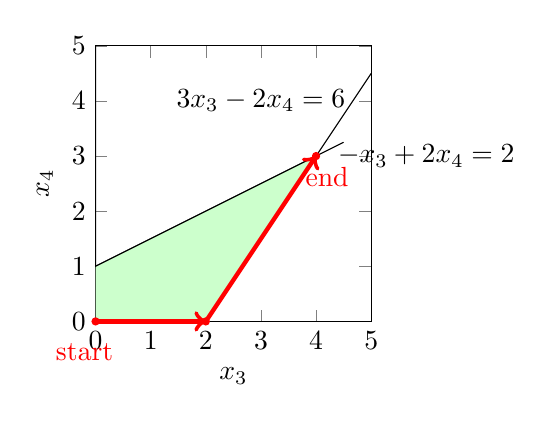
\begin{tikzpicture}[x=0.7cm,y=0.7cm]
	%\pgfplotsset{my style/.append style={ axis x line=middle, axis y line=middle, axis equal }}

	\begin{axis}[anchor=origin,         xlabel=$x_3$,
	ylabel=$x_4$,
	xtick={ 0,..., 5},
	ytick={ 0,..., 5},
	xmin=0,
	xmax=5,
	ymin=0,
	ymax=5,
	x=0.7cm, y=0.7cm,
	];
	\addplot[domain=0:4.5]{0.5*x+1};
	\addplot[domain=2:5]{1.5*x-3};
	%              \addplot[domain=-1:3,-,red]{-x+1};


	\end{axis};
	\node at (6,3) {$-x_3+2x_4 = 2$};
	\node at (3,4) {$3x_3-2x_4 = 6$};
	%              \node[red] at (4,0) {$x_3+x_4=1$};
	\draw[fill=green!20] (0, 0) -- ( 2, 0) -- (4,3) -- (0,1) -- (0,05);
	\node[circle, minimum size=3pt,inner sep=0pt, fill=red] at (0,0) {};
	\node[circle, minimum size=3pt,inner sep=0pt, fill=red] at (2,0) {};
	\node[circle, minimum size=3pt,inner sep=0pt, fill=red] at (4,3) {};
	\node[below, red, ultra thick] at (-0.2,-0.2) {start};
	\node[below, red, ultra thick] at (4.2,3) {end};
	\draw[->, red, ultra thick] (0,0) -- (2,0);
	\draw[->, red, ultra thick] (2,0) -- (4,3);
	\end{tikzpicture}

}
{

	找初始解,就是随便找一个顶点,怎么通过计算找一个顶点,任意一个
	顶点(0, 2, 0)带进去,变成一个完整解。都带进去之后,
	只找那些非零的解对应的列,也就是基。什么是顶点,顶点就是一个
	基。
}
{
	 \begin{figure}[htb]%
	 	\begin{center}%
	 		\begin{minipage}{0.3\textwidth}%
	 			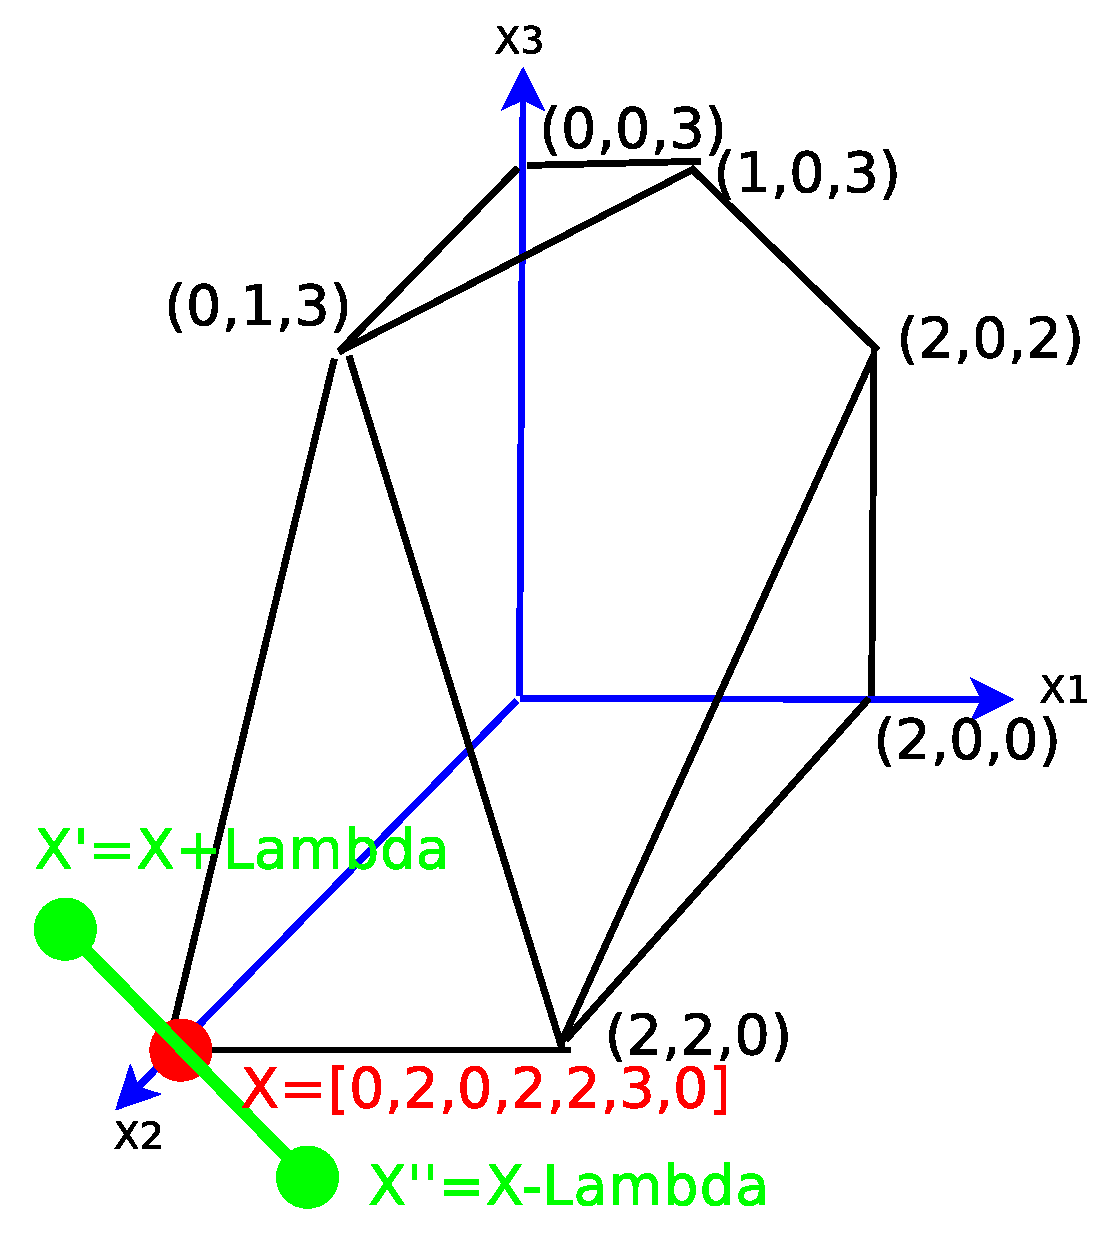
\includegraphics[width=1.0\textwidth]{L8-LPexample3Dvertex.eps}%
	 		\end{minipage}%
	 		\quad
	 		\begin{minipage}{0.36\textwidth}
	 			\includegraphics[width=1.0\textwidth]{L8-LPexample3Dvertexmatrix.png}%
	 		\end{minipage}%
	 	\end{center}
	 \end{figure}
}
{

	开始看第三个问题,第一个问题只管顶点就可以了,第二个问题顶点
	怎么找,就是找a的基,找基很简单,高斯消元法可以解决,现在
	回答第三个问题。如果当前解不太好,要improve,找和他相邻的一个
	解,找相邻的顶点,问题是怎样从一个顶点到另一个顶点呢,直观上
	看就是经过一条边,走合适的距离,怎么实现。
}
{
	\begin{figure}[htb]
		\includegraphics[width=2in] {L8-LPexample3Dstep2.eps}
	\end{figure}
}
{

	看一个例子就很清楚了,从(2, 0, 0)开始,完整带入求出完整解,
	非零列挑出来,线性无关,构成基。其他向量可以用基表示,表示唯一,
	其他写成这样,系数拿出来,可以看出,系数恰好对应一条边。
	(0, 0, -1, 1, 0, 1, 1),在三维空间,(0, 0, -1),
	向下方向,就是这条边,沿这条边走合适的距离,就是(2,0,0),
	走一段距离,$x^{\prime}$沿着$\lambda$走$\theta$ 距离,设
	$\theta=2$,后面解释为什么,带进去看看。(2, 0, 2),
	恰好是这个点,也就是说,我们思路很清晰,一开始给定顶点,
	蓝色的对应一组基,这是第一步,第二步,其他非基向量可以
	表示成基的线性组合,系数恰好对应边的方向,我们只需要沿着边
	走合适的距离就会到达一个顶点。
}

{

	严格的证明一下。x是一个顶点,顶点对应这组基,考察一个非基向量,
	非基向量$a_{e}$表示成基的组合,计算沿这个方向走多远,就是
	$\theta$,先按式子计算,得到一$\theta$,得到$x^{\prime}$对应
	一个顶点,每个顶点都对应一个基,新的顶点对应的基就是
	$B^{\prime} = B - {a_{l}} + {a_{e}}$.
}

{

	下面证明一下,证明2页slides。原先$x$是可行解,
	$ax = b$是满足的,拆成向量的形式,把绿色的
	$a_{e}$拆成基的线性组合,上面式子减去下面式子的
	$\theta$倍,这个式子是满足的,新得到的解
	$x^{\prime}_{i} = x_{i} - \theta\lambda_{i} $,
	证明新的解是可行解,可行解满足2个条件,一个是
	$ax = b$,一个是$x \geq 0$,现在只需证明第二个条件,
	分两种情况讨论,一种是所有$\lambda_{i} \leq 0$,
	所有的$x_{i} \geq 0,\theta$ 取正数,就能满足条件。
	第二种情况是,存在$\lambda_{i} > 0$,不能把$\theta$
	取的太大,否则某些$x_{i} < 0$,设置$\theta=\min_{\mathbf{a}_i\in \mathbf{B}, \lambda_i > 0} \frac{ x_{i} } { \lambda_i } = \frac{ x_{l} } { \lambda_l }$
	推导如下:
	\begin{eqnarray*}
		x_{i} - \theta\lambda_{i} \geq 0 \\
		x_{i} \geq 0 \\
		\Rightarrow \theta \leq \frac{x_{i}}{\lambda_{i}}
	\end{eqnarray*}
	$\theta$至多设置这么大,达到最大的向量给予下标$l$,
	这里面e代表enter,l代表leave。看一下例子,只用考虑
	$\lambda$中大于0的位置,$\theta$至多是多少可以算出来。
	在这里$\theta = 2, l = 4$.这样取了之后,$x^{\prime}$
	对应一个可行解。满足上面2个条件。

}
{
	再从具体的例子看一下,$\theta$的设置是从这个点
	出发,走多远恰好到一个顶点。刚才$\theta = 2$,假如
	$\theta = 3$,直观上沿这个点走3步,走出去,不在可行解
	的区域内。反应到式子里,具体就是
	$x'=x-\theta \lambda$,刚才$\theta$至多是2,如果取
	3的话,导致$x'$存在分量小于0.我们要求所有x的
	分量都是大于等于0的。所以不是可行解。
}
{
	 \begin{figure}[htb]%
	 	\begin{center}%
	 		\begin{minipage}{0.45\textwidth}%
	 			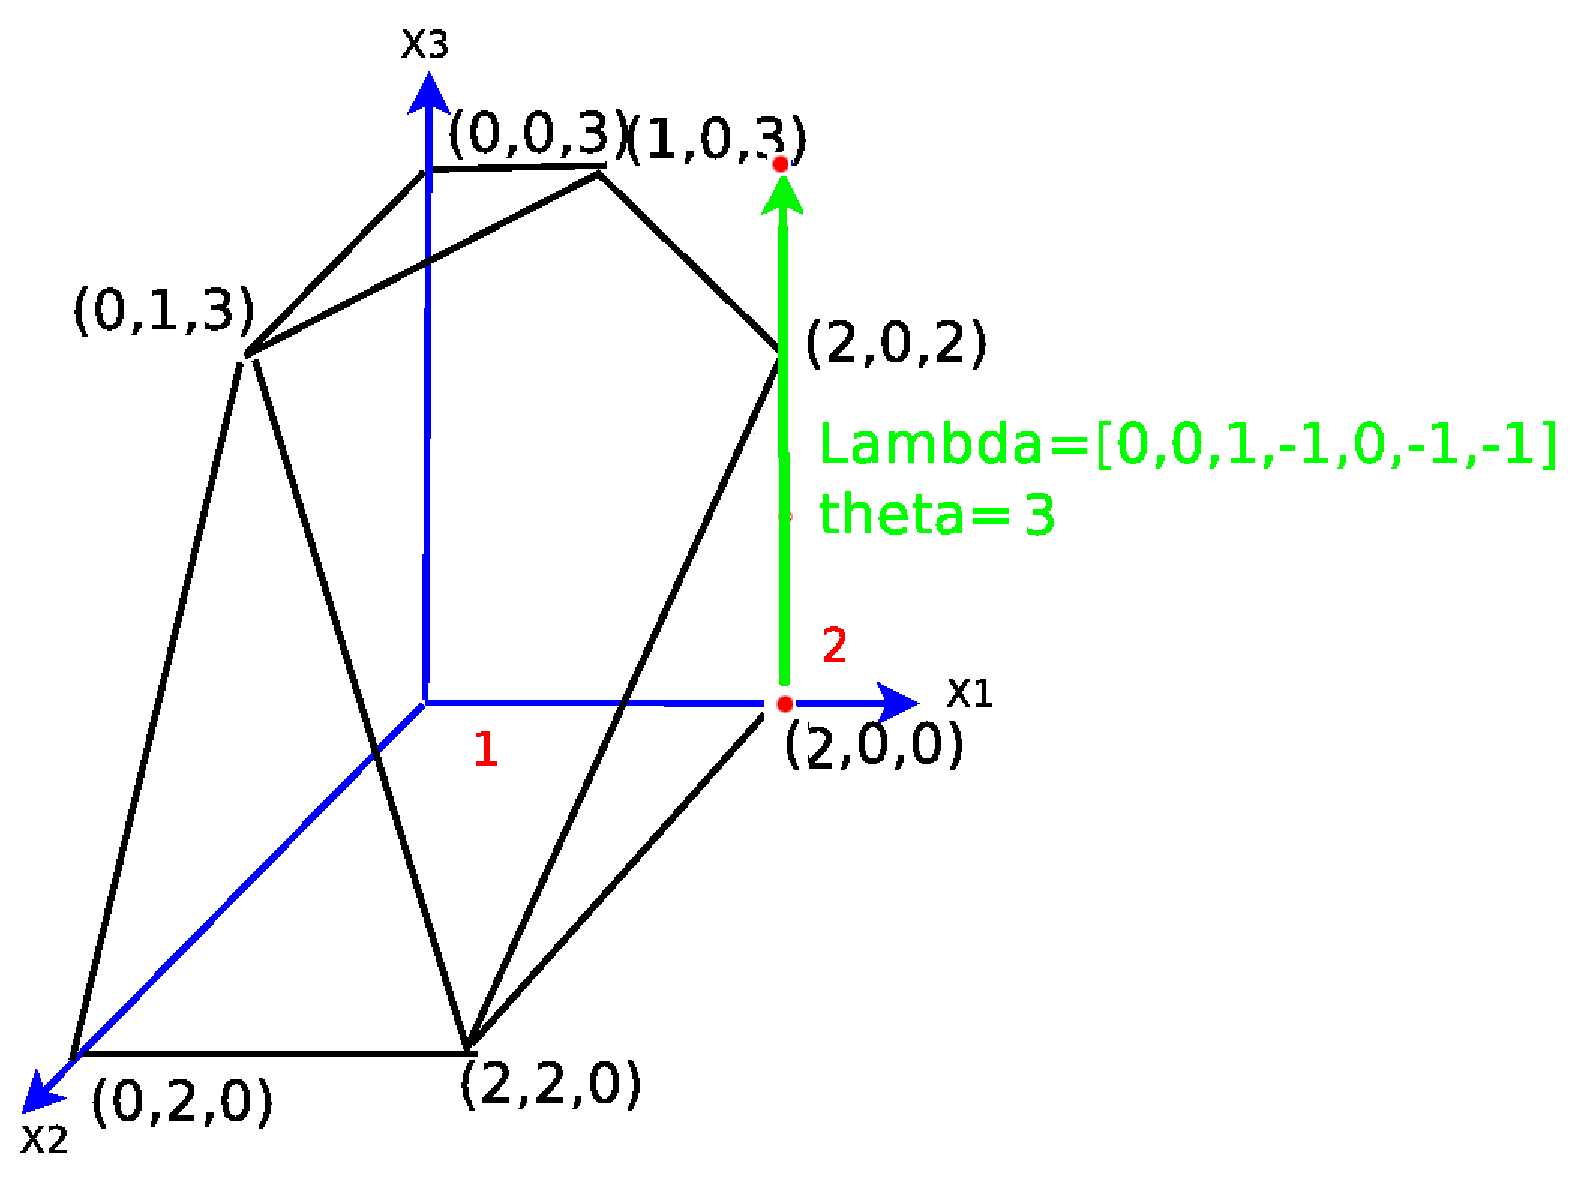
\includegraphics[width=1.0\textwidth]{L8-LPexample3Dstep2theta3.eps}%
	 		\end{minipage}%
	 		\quad
	 		\begin{minipage}{0.45\textwidth}
	 			\includegraphics[width=1.0\textwidth]{L8-LPexample3Dedgematrix.png}%
	 		\end{minipage}%
	 	\end{center}
	 \end{figure}
}
{
	再看,如果沿着这个方向走,只走一步,直观上看没有到达这个顶点,
	在这个边的中间,$\mathbf{x'=x-\theta \lambda}$不是一个顶点,也可以从
	数值上面看,取出非零列,是线性无关的,构成一个基,现在他有5个,肯定不是
	一组基。现在证完了,从x出发,沿一个方向走一定的步数,到达
	一个可行解。
}
{
	下面说明,这个可行解沿边走2步,必定到达一个顶点,对应一组
	基,怎么证明他是一个顶点呢?只需要证明$x^{\prime}$的非零列
	对应的就是一组基,是线性无关的。换句话说,我们想证明:
	在这个例子中,新的一组基怎么得到的,绿色的$a_{3}$放进来,
	$a_{4}$拿出去, $\textcolor{blue}{a_1}, \textcolor{green}{a_3}, \textcolor{blue}{ a_6}, \textcolor{blue}{a_7}$对应一组基,怎么证明?
	假如说不是一组基,是线性相关的,存在一组不为0的数,使得
	$d_1   \textcolor{blue}{\mathbf{a}_1} + d_3    \textcolor{green}{\mathbf{a}_3} +  d_6   \textcolor{blue}{\mathbf{a}_6} +  d_7   \textcolor{blue}{\mathbf{a}_7}  = 0$,注意$a_{3}$原先是非基向量,可以用原来的基唯一线性表示,
	带进去,得到新的等式,而原来的基是线性无关的,所以系数都为0,
	因此,得到新的基也是线性无关的。\\
	总结一下,一组非基向量表示成基向量的组合,系数就是方向,
	沿这个方向走多远呢,只要算一下$\theta$就行,走固定长度之后
	必定是一组基,证明就是刚才上面的过程。

}
{
	现在回顾一下,刚才讲的,随便给的初始解后,把基标出来,
	现在,沿着一条边到达一个顶点,得到新的基,原先的基去掉
	一个,新添加一个向量。看下面的例子,蓝色是旧的基,绿色是
	新添加的基,把这种操作叫做旋转pivot。蓝色是出基的向量e,
	绿色的是入基的向量l,后面讲解pivot如何实现。关于pivot的
	由来,翻译有,旋转,quicksort中的枢纽元,很古怪的用法。
	不好翻译。小布什的US pivot china。关于南海的讲话,重返亚太。

}
{
	刚才说,从任意一个顶点选择一条边,可以到达一个顶点,边
	对应非基向量,拆了之后,$\lambda$对应边的方向,红色非基向量
	表示成蓝色的线性组合,系数对应边。从(2,0,0)出发,可以到达
	三个方向,(有一个方向没画),沿着那个方向走?试试看?
	到达$x',x''$怎么样。

}
{
	 \begin{figure}[htb]%
	 	\begin{center}%
	 		\begin{minipage}{0.43\textwidth}%
	 			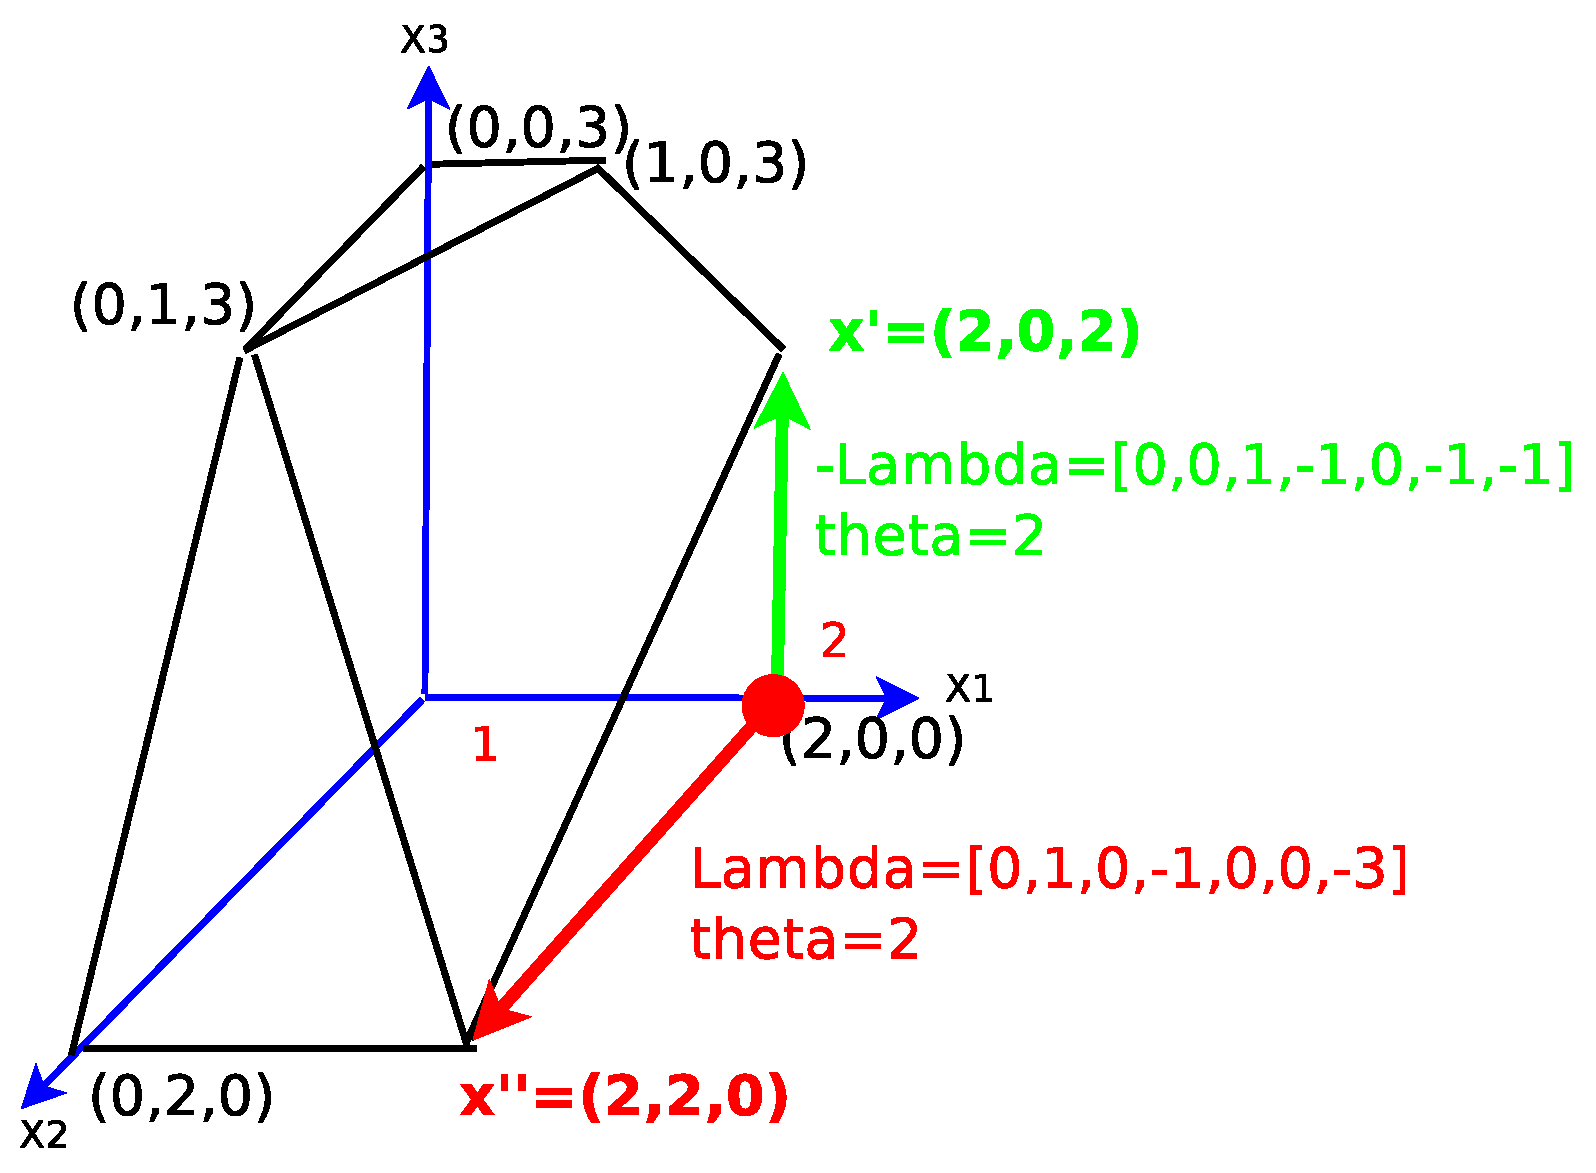
\includegraphics[width=1.0\textwidth]{L8-LPexample3Dstep2twoedges.eps}%
	 		\end{minipage}%
	 		\quad
	 		\begin{minipage}{0.43\textwidth}
	 			\includegraphics[width=1.0\textwidth]{L8-LPexample3Dstep2twoedgesmatrix.png}%
	 		\end{minipage}%
	 	\end{center}
	 \end{figure}
}
{
	先说我们走到$a_{2}$,把他表示成基的线性组合,边的方向
	就是系数,设置合理的$\theta$,得到$x''$,目标函数的变化,
	考虑到目标函数值,我们的旋转就是为了改变目标函数值。
	我们不知道选择哪个点,所以看目标函数值变化。$x''$目标函数值
	是$c^{t}x'',x$是$x^{t}x$,都是已知的得到$-14\theta$,就是目标函数
	值的改变,从x到$x''$,目标函数值大幅度降低了。
}
{
	再往后看,走另一条边,也是上面的方法,到达
	$x'$,计算目标函数的改变值,这里是$-6\theta$,
	从x move $x'$,目标函数的改变是$-6\theta$。
	一般我们采用最大梯度的规则,$-6\theta$和$-14\theta$
	所以沿着边到达$x''$的方向走,这是启发式的规则,
	一般这么用,也可以不用。
}


{
	现在只剩最后一个问题了,我们会从一个顶点到另外
	一个顶点,怎么过去呢?找非基向量就可以,什么时候
	停呢?假如说我们从一个顶点x到达$x'$,看目标函数
	改进,$\mathbf{c^{T}x' - c^{T}x}$,求这个函数的差。
	\begin{eqnarray*}
		x' = x - \theta\lambda \\
		c^{T}x' - c^{T}x = -\theta c^{T}\lambda
	\end{eqnarray*}
	详细的写开,$\lambda$到底是什么,入基的c减去其他向量,
	这是目标函数的改进,一旦这个数小于等于0,以为这从x到
	$x'$后,我们得到改善,improve,我们想minimize,每次都是下降,
	当得不到改善,就停。当上面的目标函数改进大于等于0,我们
	就停。这个公式$\lambda$的形式是怎么推出来的。
	我们有好多列,蓝色的列是基,绿色的入基$a_{e}$, 出基$a_{l}$,
	有$a_{e} = \lambda_{1}a_{1} + \lambda_{2}a_{2} + \cdots
	+\lambda_{m}a_{m},\overrightarrow{\lambda} = [ \lambda_{1}, \lambda_{2},
	\cdots ,-1, \cdots \lambda_{m}]$,然后
	\begin{eqnarray*}
		x' = x - \theta\overrightarrow{\lambda} \\
		c^{T}x' - c^{T}x \\
		= -\theta c^{T}\overrightarrow{\lambda} \\
		= -\theta[ -ce + \sum_{i=1}^{m}\lambda_{i}c_{i}] \\
		\theta[ ce - \sum_{i=1}^{m}\lambda_{i}c_{i}]
	\end{eqnarray*}
	我们什么时候停呢?如果这个数对任意的非基向量都大于等于0,
	意味着带进去目标函数没有改善,我们就停了。所以,我们把
	这个数叫做检验数。检验数写成矩阵的形式就是$\mathbf{\overline{c}^T  = c^T - c_B^T B^{-1} A }$,$\lambda$替换成$B^{-1} A$,后面解释为什么进行
	替换。现在先记住!停止条件也清楚了,任意非基向量,把他
	替换成$\lambda$,带进去算出目标函数,大于等于零就停止,也就是
	最优了!
}
{
	  \begin{figure}[htb]%
	  	\begin{center}%
	  		\begin{minipage}{0.37\textwidth}%
	  			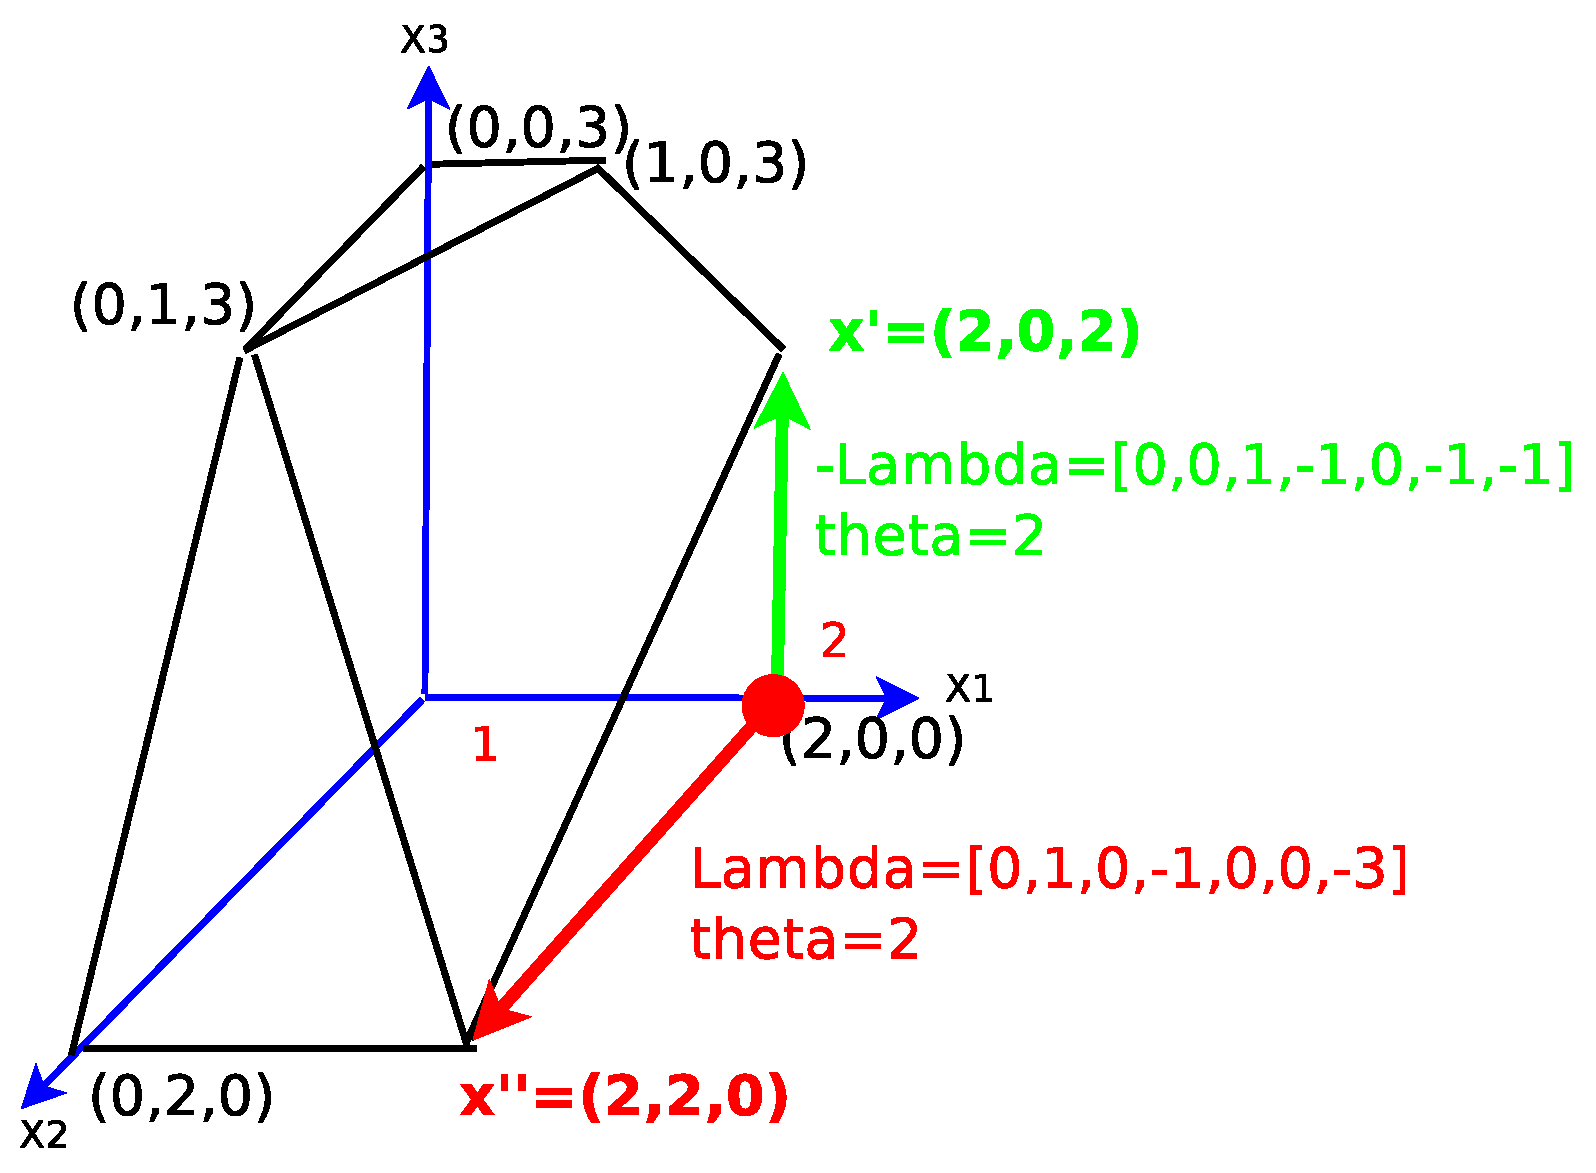
\includegraphics[width=1.0\textwidth]{L8-LPexample3Dstep2twoedges.eps}%
	  		\end{minipage}%
	  		\quad
	  		\begin{minipage}{0.42\textwidth}
	  			\includegraphics[width=1.0\textwidth]{L8-LPexample3Dstep2twoedgesmatrix.png}%
	  		\end{minipage}%
	  	\end{center}
	  \end{figure}
}
{
	为什么呢?我们严格的证明一下!考察一个线性规划,他的
	目标函数是$\min  \mathbf{c^Tx}$,约束是$\mathbf{Ax = b},
	\mathbf{x \geq 0 }$,假如说x是一个顶点,顶点就对应一组基B,
	如果算出检验数大于等于0,则x就是最优解。为什么是最优解,假如
	说我们找到一个可行解y,满足约束条件,我们可以证明任意可行解的
	目标函数都比x的目标函数大,为什么呢?因为$c^T \geq c^T_BB^-1A,
	y \geq 0, B^-1b = x_B$,任意顶点都对应一个基,顶点和基的对应关系,
	后面看例子理解,换句话说,任意可行解的目标函数值都比x的要大,所
	以是最优解。



}
{
	有点绕,大家回去后仔细看!有了这四点之后,单纯性算法就完全做完了。
}
{
	回顾一下!我把它扩展成了五点,又加了第一句琐碎的话!对线性
	规划,观察五点性质,第一点:可行解就是多面体内部,包括边界,
	最优解肯定实在定点上拿到,所以我们不用关心内部,只关心顶点,
	这比较省事!如何得到顶点呢?只要做线性变换就可以,算出基,基
	就是顶点!如果当前一个顶点不够好,想improve,在找一个点,比我好,
	怎么improve,怎么找到下一个点?沿着某一条边到下一个顶点,怎么
	沿着边走?边是什么?边就对应非基向量,拿什么时候停呢,一旦做到
	最后,一个检验数全大于零,就停。检验数是$c^T - c^TB^-1A$,为什么
	是这样?稍等一下,看这五点全有了。
}
{
	有这五点,我们就能把单纯性算法写完。写完看一下主要步骤。
	输入是矩阵A,向量b,minimize $c^Tx$,第一步调用初始化,
	找一个初始点,这个初始点,把A的基给找出来,叫做B,下标
	都放在B里面,这件事稍微有点麻烦,先假设会做这一步,待会
	会说完整的扩展,其他的都是easy。得到一个初始点,按照过去的
	规范,improve初始化,就是写一个死循环,里面先判断一下
	是不是要停,如果不存在一个非基向量,$c_{e} < 0$ 的话,检验数
	都大于等于0,我们就返回,返回的时候返回一个值。如果存在
	一个小于0,可以improve,我们随便找一个向量,也就是绿色的
	那个向量,拆成其他向量线性组合,算一下那个$\theta$,
	$\theta$等于所有的$\frac{b_{i}}{a_{ie}}$的最小值,若果$
	a_{ie} > 0$,否则$\Delta_{i} = \infty$,$\theta$去最小的
	$\Delta_{i}$,改成$\theta_{i}$,如果$\theta = \infty$,则
	是无界的,否则做一个pivot,pivot是说旧基,e为入基,l为
	出基,调用这个过程,这就是线性规划单纯性算法,里面
	有3步没解决,一个是怎么找初始点,放到最后再说,一个是
	找到一个基,我们怎么算x,接下讲解,还有一个是improve的
	时候,一个入基,一个出基,怎么操作。


}
{
	{

		\begin{footnotesize}
			{\sc Simplex}$(\mathbf{A, b, c})$
		\end{footnotesize}
		\begin{algorithmic}[1]
			\begin{footnotesize}
				\STATE $( B_{I}, \mathbf{A, b, c}, z)=$ {\sc InitializeSimplex}$\mathbf{(A, b, c)}$;
				\STATE \begin{footnotesize}\textcolor{blue}{//If the LP is feasible, a vertex $\mathbf{x}$ is returned with $B_{I}$ storing the  indices of vectors in the corresponding  basis $\mathbf{B}$; otherwise, ``infeasible'' is reported.}\end{footnotesize}
				\WHILE{ \texttt{TRUE} }
				\IF{ there is no index $e$ $(1\leq e \leq n)$ having $c_{e} < 0$ }
				\STATE{ $\mathbf{x}  = ${\sc CalculateX}$(B_I, \mathbf{A, b, c})$;}
				\RETURN{$(\mathbf{x}, z)$};
				\ENDIF;
				\STATE{ choose an index $e$ having $c_{e} < 0$ according to a certain rule; }
				\FOR{each index $i$ $(1\leq i \leq m)$ }
				\IF{$a_{ie} > 0$}
				\STATE{ $\Delta_{i} = \frac{b_{i}}{a_{ie}};$ }
				\ELSE
				\STATE{ $\Delta_{i} = \infty;$}
				\ENDIF
				\ENDFOR
				\STATE{choose an index $l$ that minimizes $\Delta_{i}$;}
				\IF{ $\Delta_{l} = \infty$ }
				\RETURN{``unbounded'';}
				\ENDIF
				\STATE{$(B_{I}, \mathbf{A, b, c}, z ) = $ {\sc Pivot}$( B_{I}, \mathbf{A, b, c}, z, e, l)$;}
				\ENDWHILE
			\end{footnotesize}
		\end{algorithmic}

}
{
	先说这一个,假如说我们知道一个矩阵A,基是B,I是index下标,
	由基确认的x是怎样的呢?是这样的?对每个$x_j$都检查一下,
	如果$x_j$不在基里面,我们说什么是基,什么是顶点?把x找
	出来,非零的那些拿出来对应一组基,话句话说,0的那些都是
	非基的,所以不在基里面的那些$x_{j} = 0$,其他那些,任意的
	一个向量的解就是b。这里写法有点绕,待会看一下例子就清楚了。
	这么写是没错的,更加鲁棒性一些,这里存疑,待会再回来看一下。
}
{
	我们讲了那么多,看个例子!假如说,我们要求这个线性规划,
	目标函数和约束如下,如何从这个约束把这个图画出来已经讲过了,
	最终是一个多面体。
}
{
	Standard form:

	\[
	\begin{array}{rrrrrrrrrrrrl}
	\min & - x_1     &-&  14 x_2    &-& 6 x_3 \\
	s.t. &   x_1     &+&     x_2    &+& x_3 & \leq & 4   \\
	&   x_1     & &            & &     & \leq & 2   \\
	&           & &            & &  x_3& \leq & 3   \\
	&           & &   3x_2     &+&  x_3& \leq & 6   \\
	&   x_1     &,&   x_2      &,&  x_3& \geq & 0   \\
	\end{array} \nonumber
	\]

	\begin{figure}[htb]
		\includegraphics[width=1in] {L8-LPexample3D.eps}
	\end{figure}

}
{
	我们先把他加一些松弛变量,变成等式约束。
}
{
	一旦做完松弛变量,我们就画了如下的一些table,单纯型算法,
	他讲线性规划,也是纸上作业,画一个表格,这个表格叫
	单纯型表,表格主体就是矩阵A,c写在上面,对一下上面的例子,
	b写在左边,有的写在右边,写在左边比较方便,左上角是目标函数
	的负数,一开始是0。单纯型表的设计,我们都很清楚,A,b,c,
	-z总共4块,事实上,我们要看的仔细一些,矩阵A始终要维护一个
	基B都是单位阵,始终要保持这一点,只要作高斯线性变换就可以,
	关键是这样保持之后,能推出很多很好的性质,很好的性质如下:
	这个矩阵A做高斯线性变换,基是B,实际上是$B^{-1}A$,
	矩阵A,基B,保持单位阵,整个矩阵乘以$B^-1$,就变成
	单位阵,这块就是$B^{-1}A$,下一页讲的更清楚。
}
{
	\begin{scriptsize}
		\begin{table}
			{
				\begin{tabular}{r|rrrrrrr}
					\hline
					& $x_1$ & $x_2$ & $x_3$ & \textcolor{blue}{$x_4$} & \textcolor{blue}{$x_5$} & \textcolor{blue}{$x_6$} & \textcolor{blue}{$x_7$}\\
					\hline
					-z= 0 & $\overline{c_1}$=-1 & $\overline{c_2}$=-14 & $\overline{c_3}$=-6 & $\overline{c_4}$=0 & $\overline{c_5}$=0 & $\overline{c_6}$=0 & $\overline{c_7}$=0 \\
					\hline
					$\mathbf{x_{B1}} = b_1'$=4 & 1 & 1 & 1 & \textcolor{blue}{1} & \textcolor{blue}{0} & \textcolor{blue}{0} & \textcolor{blue}{0} \\
					$\mathbf{x_{B2}} = b_2'$=2 & {1} & 0 & 0 & \textcolor{blue}{0} & \textcolor{blue}{1} & \textcolor{blue}{0} & \textcolor{blue}{0} \\
					$\mathbf{x_{B3}} = b_3'$=3 & 0 & 0 & 1 & \textcolor{blue}{0} & \textcolor{blue}{0} & \textcolor{blue}{1} & \textcolor{blue}{0} \\
					$\mathbf{x_{B4}} = b_4'$=6 & 0 & 3 & 1 & \textcolor{blue}{0} & \textcolor{blue}{0} & \textcolor{blue}{0} & \textcolor{blue}{1} \\
					\hline
				\end{tabular}
			} %{}%
		\end{table}
	\end{scriptsize}

}
{
	为什么单纯型表这样设计?为什么基对应的矩阵是
	单位阵,原始的矩阵A放在这,基的叫做B,非基的
	叫做N,对应的左边是向量b,上面是c,c也分块,一个
	叫$c_{B}$,一个叫$c_{N}$,这个很简单!假如说B刚开始
	不是单位阵的形式,这样不太好!我们先把他变成单位阵,
	整个矩阵乘以$B^-1$就行了,所有向量全部乘$B^-1$ 就行。
	然后变成$B^{-1}B$单位阵, $B^{-1}N $,上面也参与
	行变换,$c_{B} = 0$,仔细看一下右上角变成什么,
	$c_{i}$要变成0,要用下面的单位阵乘以$c_{i}$,再
	减去上面的就变成0,依次累加,右上角就是
	$c^{T}_{N} - c^{T}_{B}B^{-1}N$,左上角就是
	$-c^{T}_{B}B^{-1}b$.矩阵A,得到基是B,要转换为单位阵,
	好处很多,变成单位阵就是所有乘以$B^{-1}$,如上变换,怎么
	达到这一点,就是高斯行变换,线性代数里面有讲解。
	上面的c也加入高斯行变换,每列分别减去下面单位阵的
	$c_{i}, 1 \leq i \leq m$倍,就变为0,就是乘以$c^{T}_{B}$,然后减去。
	左边也要进行高斯行变换,注意左上角跟右上角的对应关系。
	这就是为什么在单纯型算法里面要千方百计的保证对应基
	为单位阵,单位阵带来好处,b,c,z是固定的。
	$B^{-1}b$对应顶点,$c^{T}_{b}B^{-1}b$对应目标函数值,
	$c^{T}_{N} - c^{T}_{B}B^{-1}N$对应检验数。分离的形式好理解,
	矩阵的形式需要仔细思考,矩阵的乘法怎么理解!
}
{
	\begin{figure}[htb]
		\centering
		\includegraphics[width=4.6in] {L8-LPABC1-ABC2.png}
	\end{figure}
}
{
	最后说一件事,就是pivot。pivot是说一开始得到一个顶点,
	把他对应的基都画起来了,非基向量进行拆,让他入基。
	pivot直观上看就是,基已经写成单位阵的形式,上面的对应的
	c都是0,非基的向量不一定是单位阵,最终想让他入基,把他变成单位阵,
	单位向量,怎么做,就是高斯行变换,看一下伪代码的意思,选定入基
	和出基,入基变成单位向量,然后高斯行变换,左边的
	b也要变,写的比较绕,实际上很简单,仔细理解一下。
}
{



		\begin{figure}
			\includegraphics[width=4.2in] {L8-LPpivoting.png}
		\end{figure}

		{\sc Pivot}$( B_I, \mathbf{A, b, c}, z, e, l)$
		\begin{algorithmic}[1]
			\begin{small}
				\STATE{\textcolor{blue}{//Scaling the $l$-th line}}
				\STATE{ $b_{l} = \frac{b_{l}}{a_{le}}$;}
				\FOR{$j = 1$ to $n$}
				\STATE{ $a_{lj} = \frac{a_{lj}}{a_{le}}$;}
				\ENDFOR
				\STATE{\textcolor{blue}{//All other lines minus the $l$-th line}}
				\FOR{$i=1$ to $m$ but $i \neq l$}
				\STATE{ $b_{i} =  b_{i} - a_{ie}  \times b_{l}$;}
				\FOR{ $j=1$ to $n$ }
				\STATE{ $a_{ij} = a_{ij} - a_{ie} \times a_{lj}$; }
				\ENDFOR
				\ENDFOR
				\STATE{\textcolor{blue}{//The first line minuses the $l$-th line}}
				\STATE{$z = z - b_{l}\times c_{e}$};
				\FOR{ $j=1$ to $n$ }
				\STATE{ $c_{j} = c_{j} - c_{e} \times a_{lj}$; }
				\ENDFOR
				\STATE{\textcolor{blue}{//Calculating $\mathbf{x}$}}
				\STATE{$B_{I} = B_{I} - \{l\} \cup \{e\};$}
				\RETURN{ ($B_{I}, \mathbf{A, b, c}, z$)};
			\end{small}
		\end{algorithmic}

}
{
	看个例子,这样大家的困惑得会解决一些!

}
{
	\begin{figure}[htb]
		\centering
		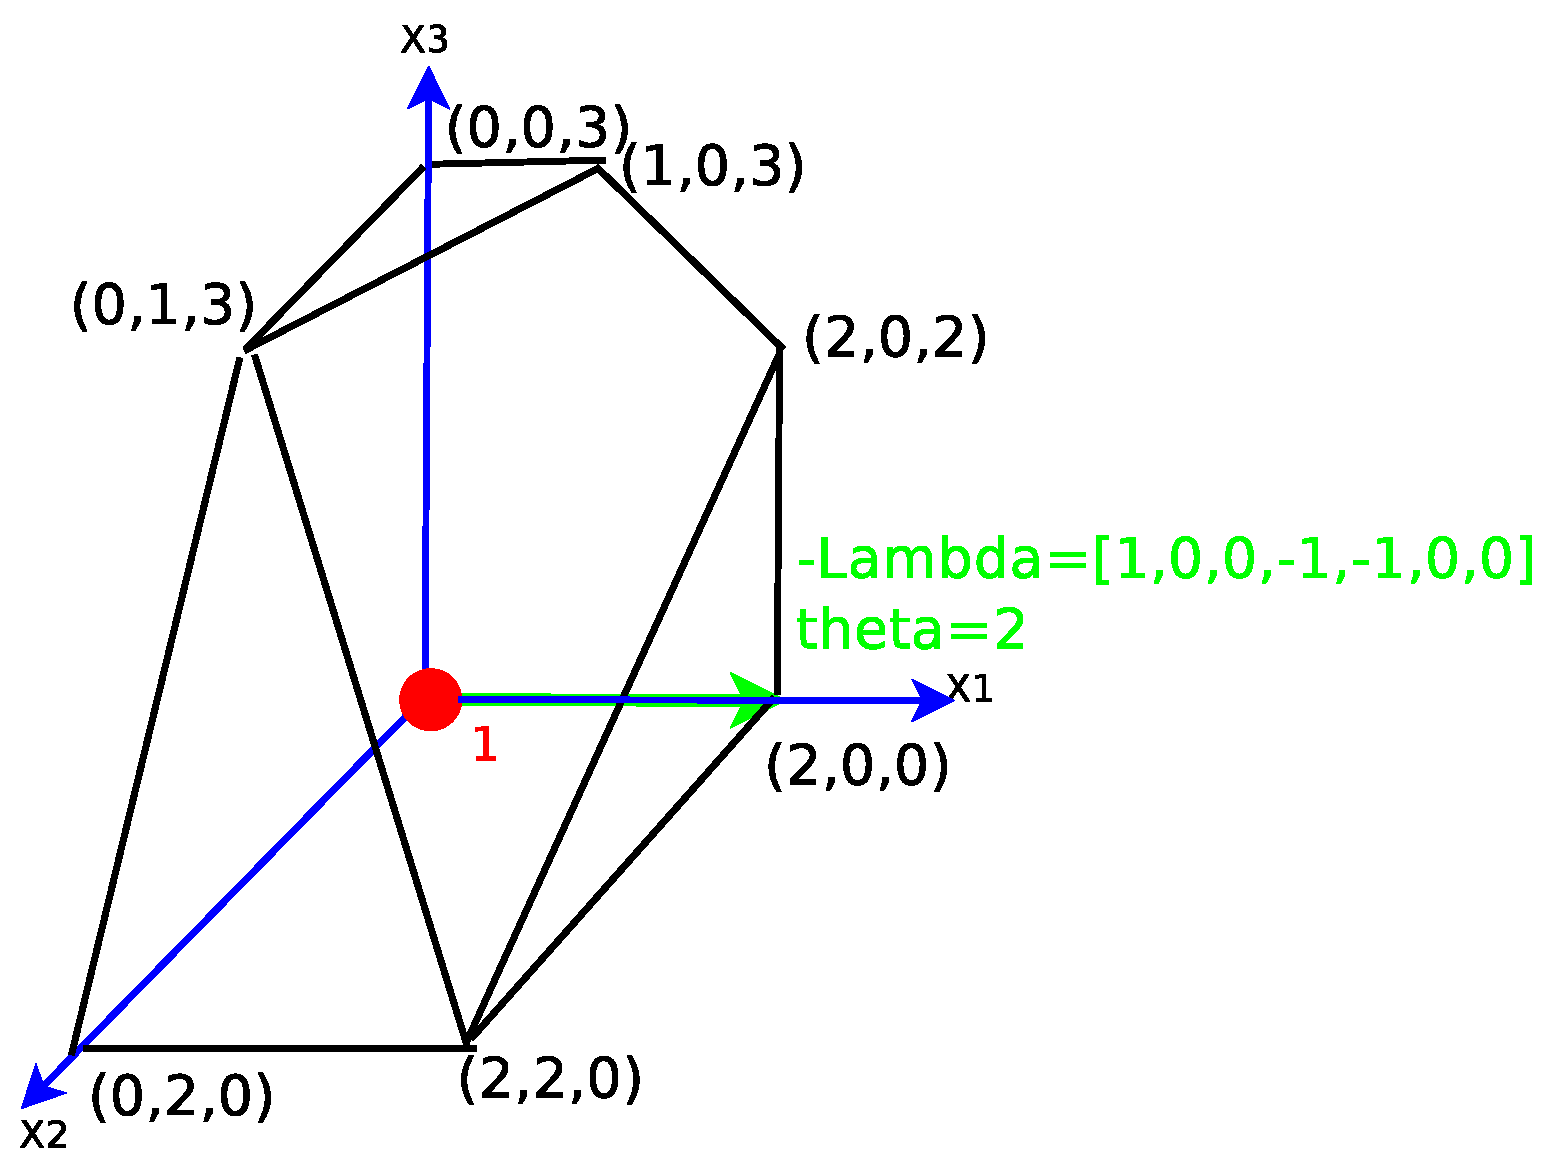
\includegraphics[width=1.4in] {L8-LPexample3Dstep1.eps}
	\end{figure}
	\begin{table}
		{
			\begin{tabular}{r|rrrrrrr}
				\hline
				& \textcolor{green}{$x_1$} & $x_2$ & $x_3$ & \textcolor{blue}{$x_4$} & \textcolor{blue}{$x_5$} & \textcolor{blue}{$x_6$} & \textcolor{blue}{$x_7$}\\
				\hline
				-z= 0 & $\overline{c_1}$= \textcolor{green}{-1}  & $\overline{c_2}$=-14 & $\overline{c_3}$=-6 & $\overline{c_4}$=0 & $\overline{c_5}$=0 & $\overline{c_6}$=0 & $\overline{c_7}$=0 \\
				\hline
				$\mathbf{x_{B1}} = b_1'$=4 & \textcolor{green}{1} & 1 & 1 & \textcolor{blue}{1} & \textcolor{blue}{0} & \textcolor{blue}{0} & \textcolor{blue}{0} \\
				$\mathbf{x_{B2}} = b_2'$=2 & \textcolor{red}{1} & 0 & 0 & \textcolor{blue}{0} & \textcolor{blue}{1} & \textcolor{blue}{0} & \textcolor{blue}{0} \\
				$\mathbf{x_{B3}} = b_3'$=3 & \textcolor{green}{0} & 0 & 1 & \textcolor{blue}{0} & \textcolor{blue}{0} & \textcolor{blue}{1} & \textcolor{blue}{0} \\
				$\mathbf{x_{B4}} = b_4'$=6 & \textcolor{green}{0} & 3 & 1 & \textcolor{blue}{0} & \textcolor{blue}{0} & \textcolor{blue}{0} & \textcolor{blue}{1} \\
				\hline
			\end{tabular}
		} %{}%
	\end{table}

}
	{
		三步骤,第一步
	找一个初始点,第二步找谁进去,第三部进去之后再变一次,
	第四部就是什么时候停。公式比较多,看的麻烦!就解
	前面那个线性规划的例子!画出单纯型表,写上A,b,c,
	z,没什么问题。第一步找一个初始点,初始点就是基,
	蓝色的就是基,而且就是单位阵,基对应的顶点写成
	矩阵的形式就是$\mathbf{x=\left[\begin{array}{c}\mathbf{B^{-1}b}\\\mathbf{0}\end{array}\right]}= [ 0, 0, 0, 4, 2, 3, 6 ]^T$,非基的都是0,基对应的
	就是b,可以写出x。找到基了,基就是顶点,这点不太好,然后进行
	改进,随便找个非基向量,绿色的,让他入基,沿着他
	走多远呢?随便找一列,只要上面对应的c小于0,就可以。
	为什么小于0,刚才说了,先不管他。这就是入基,然后是
	出基,这一列里面找大于0的,除法计算最小的$\theta$值,
	对应的行的单位阵也就是旧基里面为1的那一列为出基,
	单纯型算法3步,第一步:初始点:基,第二部:while\{t\}
	找一个负的$c_{i}$,用$\frac{b_{i}}{coef}$,找最小的,
	然后行变换。如果找不到负的就结束。在这个例子里面接下
	来就是做高斯行变换,新的基就产生了,跟原来不一样。
	对应图里面就是,原始的点事$x_{1}$,走到右边那个点。
	接着再找c里面谁是负的,这一列里面找正的,然后做
	高斯行变换,写程序比较简单。这里面插一句话:
	这里b是0,比较奇怪,导致$\theta = 0$,这很特殊,
	也就是说当前点沿着找的的方向走0步,还是自己这个点。
	这是什么意思?这可能带来危险!可能一直在这个点呆着,
	这种情况叫做退化!接下来往下走,最后所有的c都是大于等于
	0的,停了,当前点是最优点。最优点的值是什么?基对应相应
	的b,非基都是0,所以写程序比较简单!但是,为什么能方便的
	写程序实现单纯型算法呢,就是因为单纯型表有那些优秀的性质。
	始终把基表示成单位阵,b对应解,上面的c对应检验数,左上角
	是目标函数值,那一页slides就是最核心的。


}
{
	在单纯型算法过程当中,我们有可能在一个点不断的呆着。
	因为$\theta = 0$,怎么办?有很多办法处理这个事情,处理的
	规则暂时不讲,大家感兴趣可以看一下附加的slides。先往下讲。
}
{
	对单纯型算法强调几点:第一点,写程序是很easy 的,只是背后的
	知识,为什么要这么实现,讲课的难点在这里,为什么矩阵是
	这样的。第二个比较难的地方还是在矩阵,很多的术语写成分离
	的形式很好理解,但写成矩阵的形式,不好理解。熟悉一下矩阵乘法
	表达的意思。剩下的困难就不多了。这次课后有个作业实现单纯型
	算法,第一因为单纯型算法非常经典,第二这个套路在其他地方很有用
	。第三点,学生实现过后,我现在很多研究,在基因组上的线性规划,
	基因组上有上千万个点$x_{i}$,调用所有的软件包都不行。因为
	内存空间占用太大,但是结构很奇怪!这里说明为什么让大家练的原因?
	因为起码对我的工作是有用的,对大家将来有可能有用。基因组
	是一个长长的线段,上面有一些点$x_{i}$,点的数目非常多,10M,
	上千万左右,知道有些点之间的距离$d_{ij}$。把整体的$x_i$求出来。
	线性规划如下:
	\[
	\begin{array}{ll}
	min & E \\
	s.t. & x_{i} - x_{j} = d_{ij} + \varepsilon_{ij} \\
	& |\varepsilon_{ij}| \leq E
	\end{array}
	\]
	$\varepsilon_{ij}$是误差,$d_{ij}$已知,使误差最小化。
	最简单的,还没用二次平方误差!数据量比较大!按道理来说,
	应该是mse准则!现在线性的都搞不定,不能用平方!
	这个线性规划,上千万的时候,现有的包都搞不定!
	gourbi,glpk,都不行!要用特定的算法解决!这个样子比较奇怪,
	这样单纯型表的矩阵A是极度稀疏的,而且维数很大!内存
	根本放不下。我们要重新编写。
}
{
	下面来看一个例子!这个例子比过去的要直观一些!是下面
	这样子的\[
	\begin{array}{rrrrrrl}
	\min & - x_1 & - & x_2 & \\
	s.t. &   x_1 & - & x_2 & \leq & 1   \\
	& - x_1 & + & x_2 & \leq & 1   \\
	&   x_1 &,  & x_2 & \geq & 0   \\
	\end{array} \nonumber
	\]
	在图上看一下约束是怎么样的,具体的对应关系!这个
	解区域有点问题,不是封闭的!把目标函数的等高线画出来。
	可以看到目标函数可以取到负无穷,这是在图上直观的看法,
	那运行单纯型算法会怎么样呢?
}
{
	\begin{figure}
		\includegraphics[width=2in]{L8-unboundedlp.png}
	\end{figure}
}
{
	先把他写成松弛型,添加松弛变量,变成等式约束。

}
{



		\begin{small}
			Standard form:
			\[
			\begin{array}{rrrrrrl}
			\min & - x_1 & - & x_2 & \\
			s.t. &   x_1 & - & x_2 & \leq & 1   \\
			& - x_1 & + & x_2 & \leq & 1   \\
			&   x_1 &,  & x_2 & \geq & 0   \\
			\end{array} \nonumber
			\]
			Slack form:
			\[
			\begin{array}{rrrrrrrrrl}
			\min & - x_1 &-& x_2   \\
			s.t. &   x_1 &-& x_2 &+& x_3 & &     & = & 1   \\
			& - x_1 &+& x_2 & &     &+& x_4 & = & 1   \\
			&   x_1 &,& x_2 &,& x_3 &,& x_4 &\geq & 0 \\
			\end{array} \nonumber
			\]
		\end{small}

}
{
	画出单纯型表,写出矩阵的形式,照抄,很简单!
	第一步先找基,这很简单,松弛变量天然的就是一组
	基。由基可以反解出x,然后开始while循环,先找c
	里面小于0的列,对应A里面的正数,求出$\theta$的
	最小值!负的不管。做高斯行变换,入基和出基。
	得到新的基。再重复,找c里面负的!找到了,
	然后A里面对应的没正的,原来找正的,是因为走太远
	会出圈,现在全是负的。
	\[
	\begin{array}{llll}
	x & = & [1, 0, 0, 0] &\\
	\overrightarrow{\lambda} & = & [-1, 0, 0, 0] &\\
	x' & = & x - \theta\overrightarrow{\lambda} &\geq 0
	\end{array}
	\]
	直观上看,可也沿着这条边走无穷远,都是可行解!
	每走一步,目标函数都会变小,所以无界,想多小就多小!
	特征就是A里面对应的列全是小于等于0的。到现在为止,
	单纯型算法都会跑了,单纯型算法里面3块,现在解决2块,
	算法里面:找初始点,死循环,死循环里面都找有没有
	小于等于0的,若有,则沿着这个方向,找到最小的$\theta$,
	做高斯行变换就完了,现在还剩初始点怎么找?
	初始时给我们矩阵A,向量b和c,怎样找一个基,使得对应
	基的b是大于等于0的。
}
{
	最后一个问题,我们会improve,但是初始顶点怎么找?
	换句话说,让我们解$\mathbf{Ax = b}$, $\mathbf{x \geq 0}$,
	怎么解?用以前的知识能不能解?只会$\mathbf{Ax = b}$,
	但不一定满足要求!找这个点怎么做?不用线性规划是
	没法做的!过去学的那一套做不了。
}
{
	让我们看怎么做!假如说解下面的问题,找一个初始解。
	怎么办?我们把转换成解下面的辅助线性规划!辅助线性规划
	是这样子的,添加变量$x_0$,minimize$x_0$,注意这里
	变换后还是小于等于0的,再陈述一次,求解$\mathbf{Ax = b}$, $\mathbf{x \geq 0}$,
	不会做,变成解辅助线性规划,加了一个目标函数,每个约束
	都减了个$x_0$。
}
{
	为什么是这样子的?假如说原先的线性规划有可行解,
	现在加上$x_0$,其他值不变,这就是辅助线性规划的一个可行
	解。原来解满足约束,加上$x_0 = 0$后也满足新的辅助线性规划的
	约束。搞到一个可行解,就是最优解。假如说原来的L 没有
	可行解,对于任意取值,至少有一个约束不可满足,假如
	是第i行约束,那么根据辅助方程组,就有$x_0 > 0$。
	minimize$x_0$,$x_0$取不到0。辅助线性规划有解,但是解
	不是$x_0 = 0$。大家回去琢磨一下,这是非常巧妙的构造。
	上面有可行解,下面最优解肯定是0.
}
{
	那怎么解辅助线性规划呢?很简单,先加上松弛变量,变成
	松弛型。因为松弛变量天然对应基。
}
{
	\[
	\begin{array}{rrcrrrrrrrrrl}
	\min &    & &   &  \textcolor{red}{x_0}                                   &          &        &         &         & \\
	s.t. & a_{11}x_1 &+ ... &+a_{1n}x_n   &\textcolor{red}{-x_0}& \textcolor{blue}{+ s_1}&       &         &\textcolor{blue}{=}  b_1 &  \\
	& a_{21}x_1 &+ ... &+a_{2n}x_n    &\textcolor{red}{-x_0}&         &\textcolor{blue}{+s_2}&         &\textcolor{blue}{=}  b_2 &  \\
	&           & ... &                                       &  &     &    &  &  &\\
	& a_{m1}x_1 &+ ... &+a_{mn}x_n &\textcolor{red}{-x_0}&          &        &     \textcolor{blue}{+s_m}     &\textcolor{blue}{=}  b_m &  \\
	&         x_1  &, ... ,&       x_n,          &\textcolor{red}{x_0},& \textcolor{blue}{s_1},   &\textcolor{blue}{s_2}, & ...    \textcolor{blue}{s_m}   &  \geq  0   &  \\
	\end{array} \nonumber
	\]
}
{
	之后,如果所有的$b_i$都大于等于0,我们直接取他们作为基。
	其他的非基都是0,这就是可行解。
}
{
	如果有个负的,比较麻烦,不能直接作为基。作为基之后,
	不是一个可行解。怎么办呢?一旦$b_i$有负的之后,找
	$b_i$里面的最小值,负的最厉害的,其他所有的全减去负的最小
	的数,其他都是正的,自己再乘负号就行。

}
{
	具体的过程不用管,回头看看就行,先看后面的例子,就清楚了!
}
{


		\begin{algorithmic}[1]
			\begin{footnotesize}
				\STATE let $l$ be the index of the minimum $b_i$;
				\STATE{ set $B_I$ to include the indices of slack variables; }
				\IF{ $b_l  \geq 0$ }
				\RETURN{ $(B_I, \mathbf{A, b, c}, 0)$ };
				\ENDIF
				\STATE{construct $L_{aux}$ by adding $-x_0$ to each constraint, and using $x_0$ as the objective function;}
				\STATE{let $(\mathbf{A, b, c})$ be the resulting slack form for $L_{aux}$; }
				\STATE{\textcolor{red}{//perform one step of pivot to make all $b_i$ positive; }};
				\STATE{ $(B_I, \mathbf{A, b, c}, z) = ${\sc Pivot}$( B_I, \mathbf{A, b, c}, z, l, 0)$;}
				\STATE{ iterate the {\sc while} loop of {\sc Simplex} algorithm until an optimal solution to $L_{aux}$ is found; }
				\IF{ the optimal objective value to $L_{aux}$ is 0}
				\STATE{ return the final slack form with $x_0$ removed, and the original objective function of $L$ restored; }
				\ELSE
				\RETURN{ "infeasible";}
				\ENDIF
			\end{footnotesize}
		\end{algorithmic}

}
{
	给我们解下面的线性规划,首先要求一个可行解!先画出
	可行域是什么样子的。既要在上面,又要在下面,所以
	直观上是没有可行解的。
}
{

		\begin{small}
			LP $L$:
			\[
			\begin{array}{rrrrrrl}
			\min &   x_1 & + & 2 x_2 & \\
			s.t. &   x_1 & + & x_2 & \geq & 2   \\
			&    x_1 & + & x_2 & \leq & 1   \\
			&   x_1 &,& x_2 & \geq & 0
			\end{array} \nonumber
			\]
		\end{small}
		\begin{figure}
			\includegraphics[width=1.8in]{L8-LPinitialsolutionexample2.png}
		\end{figure}

}
{
	给我们线性规划,先求辅助线性规划,形式如前面讲解的
	那样,添加$x_0$,然后把辅助线性规划转换成松弛型,这都使基本
	步骤。
}
{
	接着,写出单纯型表,矩阵照抄,松弛变量是基,但是
	对应的$b_i < 0$,不是可行解,怎么办呢?所有的行
	都减去这个负的,然后自己再乘一个负号。然后就得到新基。
	且这个基对应的$b_i > 0$是可行解。所有约束都有$-x_0$,
	减去之后,除了自己有$-x_0$外,其他都没有。然后自己
	变成$+x_0$。大家体会一下基的变化!找到新基,且对应的b
	是可行解。再往下面跑一步,找一下c有没有负的,然后取一列,
	找出$\theta$,做高斯行变换。最后停了!上面的c都是大于等于
	0的,stop,得到最优解!最优解的值是$-\frac{1}{2}$,
	我们的目标函数值是0的话,意味着原始的有可行解!现在
	不是0,是负的,原先没有可行解!到现在为止,大家终于会
	本科学的东西有扩展了。$Ax = b$会做,加上限制$x \geq 0$就
	不会了,现在怎么做?变成辅助线性规划做!
	\[
	\begin{array}{ll}
	min & x_{0} \\
	s.t. & Ax + x_{0} = b \\
	& x \geq 0 \\
	& x_{0} \geq 0
	\end{array}
	\]
	所以很多时候,我们稍微加一点限制,过去的方法就不能做,
	必须要有更高级的工具才能解!
}
{
	我们再来看,刚才没有可行解,再看个有可行解的例子!
}
{

		\begin{small}
			LP $L$:
			\[
			\begin{array}{rrrrrrl}
			\min &   x_1 & + &2  x_2 & \\
			s.t. &   x_1 & + & x_2 & \leq & 2   \\
			&    x_1 & + & x_2 & \geq & 1   \\
			&   x_1 &,& x_2 & \geq & 0
			\end{array} \nonumber
			\]
		\end{small}
		\begin{figure}
			\includegraphics[width=1.8in]{L8-LPinitialsolutionexample1.png}
		\end{figure}

}
{
	稍微改一下,是这样子的!变成下面的线性规划!跟图
	进行对照,直观上看,是有可行解的!求解一下过程!
}
{
	也是刚才的步骤,构造辅助线性规划,转化成松弛型,非常easy。
}
{
	转换之后,写出单纯型表,松弛变量是基,但是基对应的b
	不是可行解,做初始化,减去负的最小的,然后自己乘以负号,
	得到新基和可行解。不断的while循环,最后一步!所有的c都是
	正的,就返回了!得到最优的可行解!对应的目标函数值是0,
	意味着辅助线性方程组的解达到最优解0.所以原始的方程是有
	可行解的。直接带进去就可以了。下一页是如何把初始可行解转化为
	转化为输入,可以暂时跳过,实现的时候比较方便,可以完全不管他。
}


{
	我们讲完单纯型算法,大家回去可以用熟悉的语言实现。
	python语言不到200行,就能实现!我们会写单纯型算法,
	实际情况,他会跑多快呢?
}

{
	这一页,大家看一下介绍,单纯型算法1949年Dantzig 提出来的,
	很多人都在用,发现很快!做高斯行变换,基要换入和换出,
	要换多少次呢?实践当中发现的次数,基本上跟m成比例。
	和n的关系很小。有人说,固定m之后,运行次数跟$logn$成比例。
	这都是实践的经验!迭代的次数跟m有关,while循环的次数,随意
	总体的运行时间是$O(m^2n)$,因为while循环每一次都要做高斯
	行变换,矩阵的规模是$mn$的,$O(m)$轮,所以是$O(m^2n)$。
	对稀疏矩阵来说,就像刚才的基因序列例子,运行时间$O(Km^\alpha n d^{0.33})$
	,K是常数,m是行数,n是线性的,d是有多少个非零元。
	看稀疏程度怎么样。
}
{
	来实际看一下,我写了个程序,随机的产生很多线性规划,
	跑glpk,跑单纯型算法,看总共要几轮结束,首先固定约束m,
	变量数不断增长,观察有多少次!随着变量增加,换入换出增加
	非常缓慢!的确很像$logn$.
}
{
	又换另外一个,假如我们固定n,约束不断的增加。每个都
	随机的产生了一堆!每个至少产生1000个。每个点都是均值!
	看到迭代的次数跟m显著增加,很像线性的$O(m)$,大概是这样的。

}
{
	但是,非常不幸的是,单纯型算法在实际生活中跑的非常快,
	基本上是$O(m^2n)$,但是不是多项式时间算法。
}
{
	这件事,直到1972年,V. Klee and G. L. Minty构造了一个稀奇古怪的
	例子,在他上面跑单纯型算法,就要花指数的时间。看一下
	例子是怎么样子的。
}

{
	具体的例子如下,有这些数学表达式,画出多面体。如下图。
	这个样子比较难画!这个稀奇古怪的多面体会导致什么情况呢?
	他总共有8个点,跑单纯型算法,所有的顶点都会遍历一次。
	看附加的slides演示。各个棱是不一样长的。每一次move都是
	下降的。总共8个顶点,都要旅行到,才可以。这是讲单纯型
	算法难点最简单的一个例子。实际的跑一下例子。的确要跑
	$2^n$的。看一下glpk是不是有进行优化。根据V. Klee and G. L. Minty
	的例子进行构造,产生最多100万个,看一下运行时间。是
	指数上升的。scrip也放在网上,可以自己运行!沿着这条线,
	是支书时间,只是存在这种可能性,glpk大概按照这条线走的。
	花了指数时间,我们怎么不让他犯错呢,加一点error,马上时间就
	降下来。
}
{
	为什么单纯型算法在实际的例子中跑的很快,只要$O(m^2n)$,
	但是的确存在一个例子,这个例子需要跑指数多的时间。这中间
	就有矛盾!怎么解决?有一个新的解决办法,叫平滑分析,平滑
	复杂度。
}
{
	平滑分析是Daniel A. Spielman, Shang-Hua Teng在2001年得出
	的分析方法。找准自己感兴趣的方向!2001年得到哥德尔奖。
	他们说单纯型算法是指数时间复杂度,但是他有多项式时间的
	平滑复杂度。换了一个度量。不用最坏时间,用平滑的,他
	就是多项式时间。
}
{
	那什么是平滑时间复杂度?讲个例子!到现在讲了3个分析方法,
	一个是平均时间分析,一个叫最坏时间分析,还有一个
	均摊分析。这3件事。平均时间分析解决最坏时间分析
	的困难,但是平均时间分析有问题。平滑时间复杂度是
	平均时间分析和最坏时间分析的一个折中。看一下画的图。
	x轴是instance例子,每个点事固定n,y轴是时间。最坏时间
	复杂度是最慢的例子,平均下来很低,average范围太广,拿不到
	所有的例子,不太可能,实际中做不动。怎么办?平滑时间复杂度
	是说稍微做点扰动,求平均,是很小的。在小邻域内做平均。
	复杂度很低。这是我们的解释,V. Klee and G. L. Minty构造的例子非常古怪,
	我们日常生活中拿到的例子,都有error,也就说现实生活中
	很难遇到V. Klee and G. L. Minty的例子,总是带点噪声的例子。
	看一下带噪声的例子!看一下有噪声会出什么事!构造一个例子。
	解$Ax = b$,A加上一个noise,用条件数解释,都一样,无法解释,
	很生动!大家做图像处理或者信号处理,总是很讨厌噪声,
	总是要想办法把噪声去掉,但是,滕老师说:“噪声是个好东西!”。
}



